\begin{figure}[htbp]
\centering
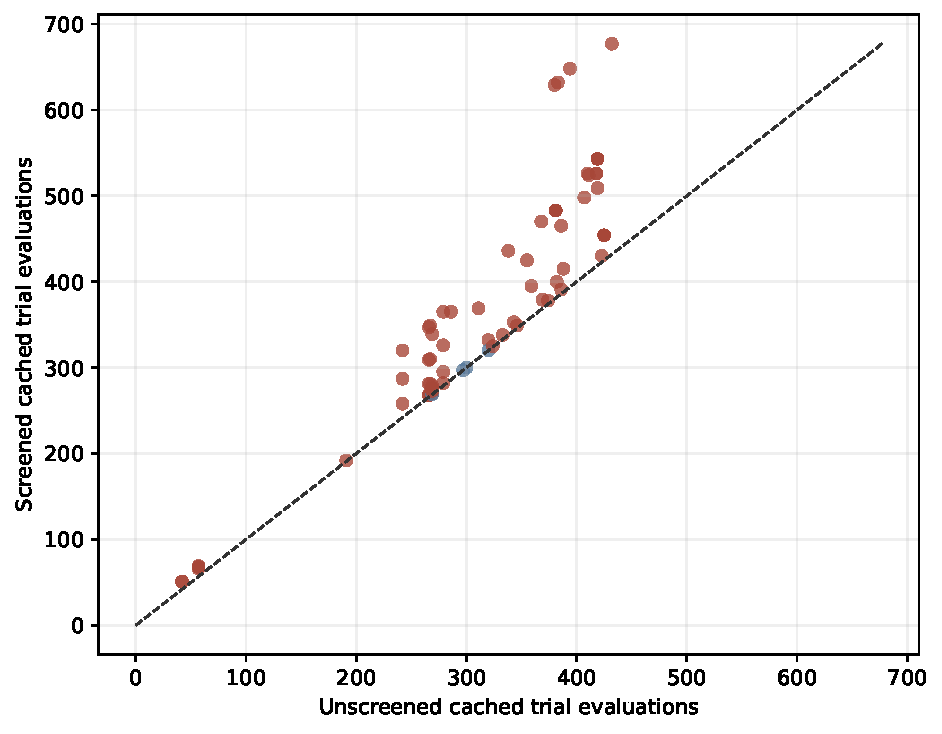
\includegraphics[width=0.92\textwidth]{figures/paired-cost.pdf}
\caption{Paired cached exact-engine evaluations for each target-mode variant; points above equality indicate added screened work.}
\label{fig:cost}
\end{figure}
\begin{figure}[htbp]
\centering
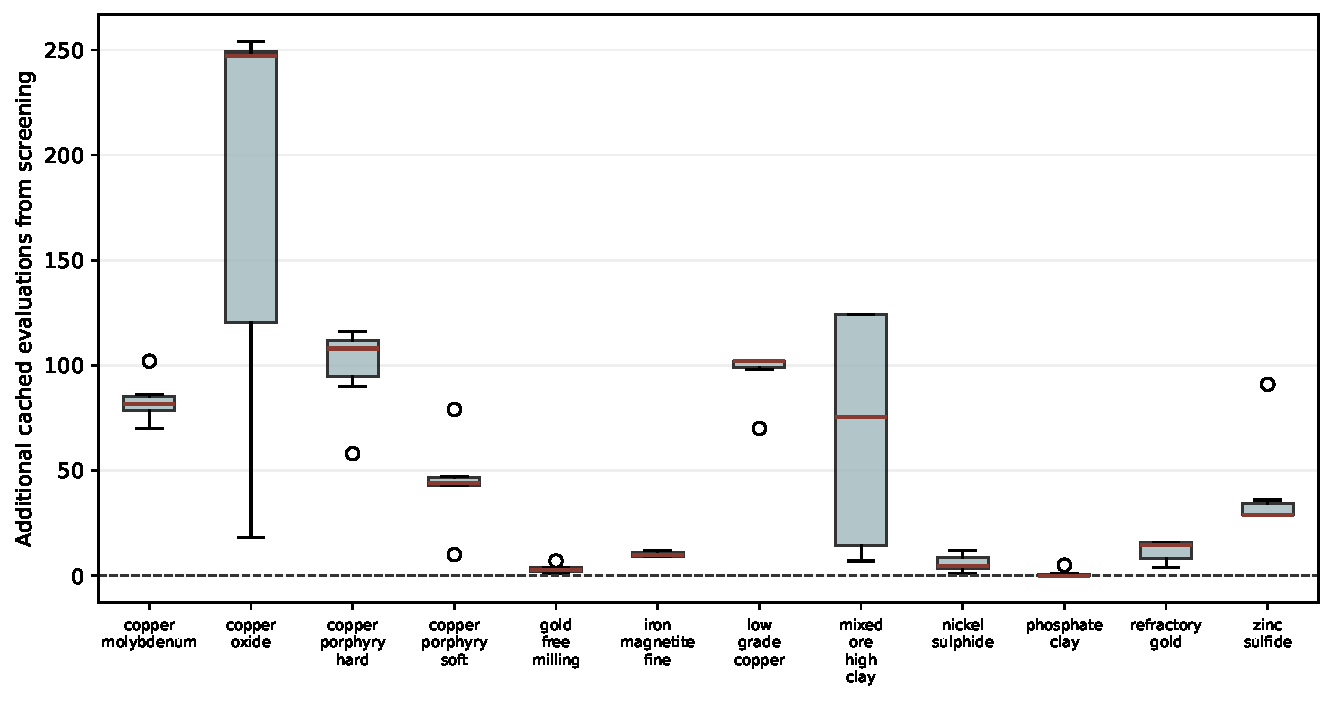
\includegraphics[width=0.92\textwidth]{figures/case-cost-deltas.pdf}
\caption{Variant-level evaluation-count changes by authored case and circuit family; positive values mean screening increased exact-engine work.}
\label{fig:case-cost-deltas}
\end{figure}
\begin{figure}[htbp]
\centering
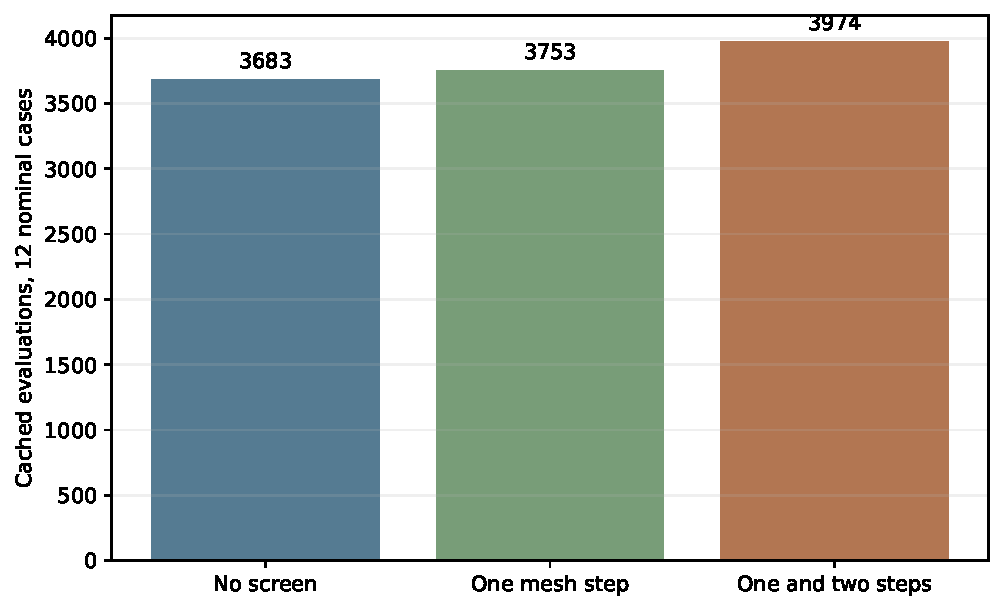
\includegraphics[width=0.92\textwidth]{figures/step-ablation.pdf}
\caption{Nominal weight-one evaluation totals across twelve authored cases under no screen, one-step screening and the full one-and-two-step policy.}
\label{fig:step-ablation}
\end{figure}
\begin{figure}[htbp]
\centering
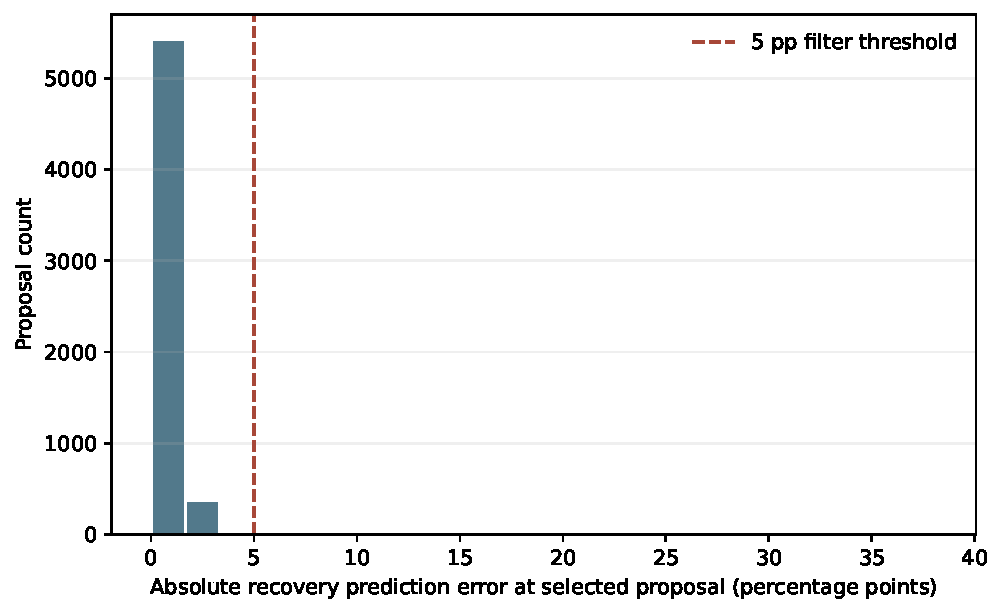
\includegraphics[width=0.92\textwidth]{figures/proposal-error.pdf}
\caption{Absolute recovery prediction error for every exact-evaluated selected proposal, with the five-point interval filter threshold marked.}
\label{fig:proposal-error}
\end{figure}
\begin{figure}[htbp]
\centering
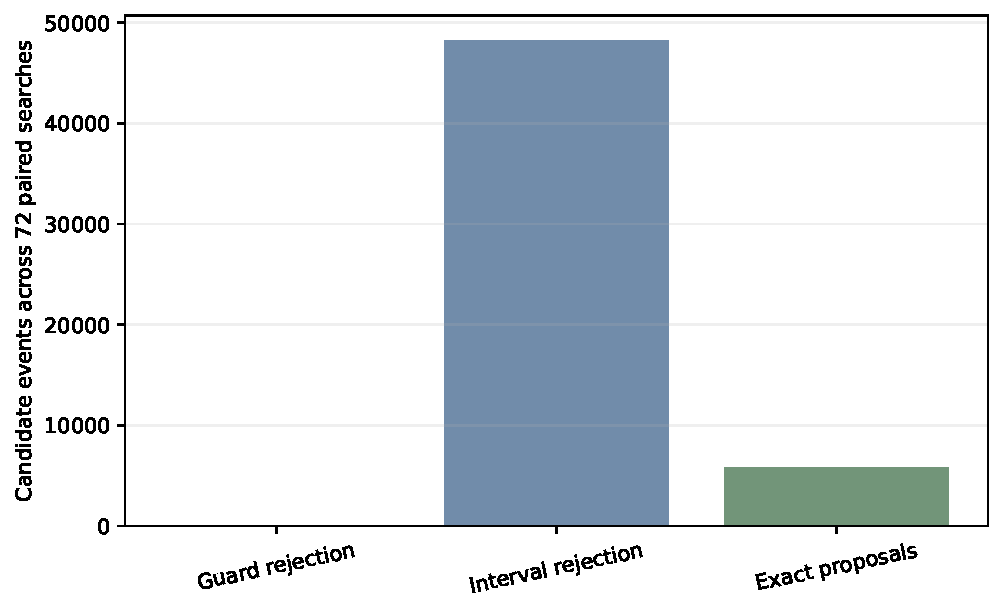
\includegraphics[width=0.92\textwidth]{figures/screen-activity.pdf}
\caption{Guard and interval rejections and proposals aggregated over the 72 paired variants; rejection totals count candidate events.}
\label{fig:screen-activity}
\end{figure}
\begin{figure}[htbp]
\centering
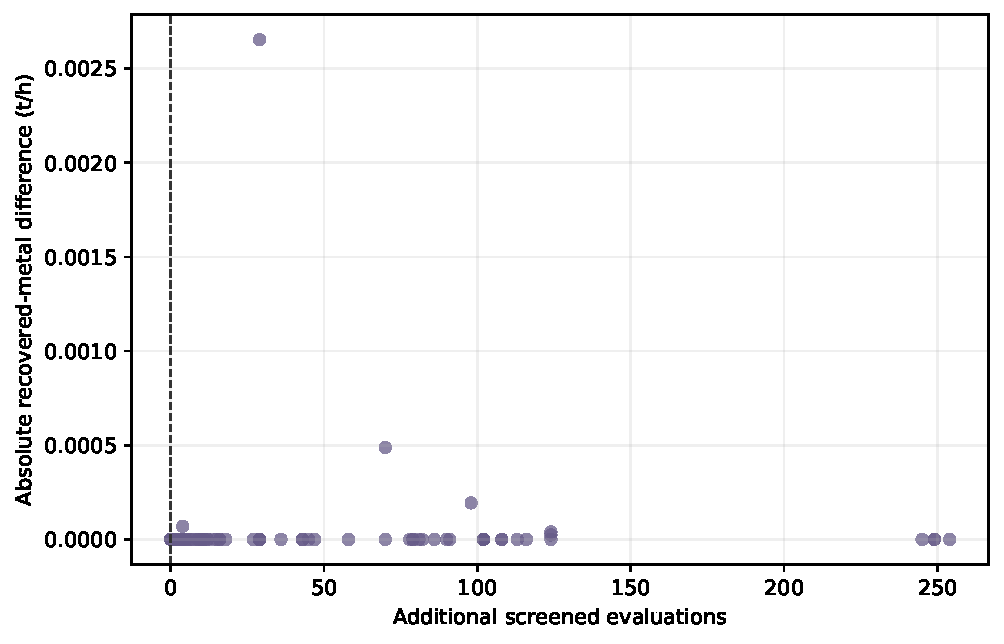
\includegraphics[width=0.92\textwidth]{figures/cost-decision.pdf}
\caption{Added exact evaluations plotted against absolute recovered-metal differences for the matched target-mode outcomes across all twelve authored cases.}
\label{fig:cost-decision}
\end{figure}
\begin{figure}[htbp]
\centering
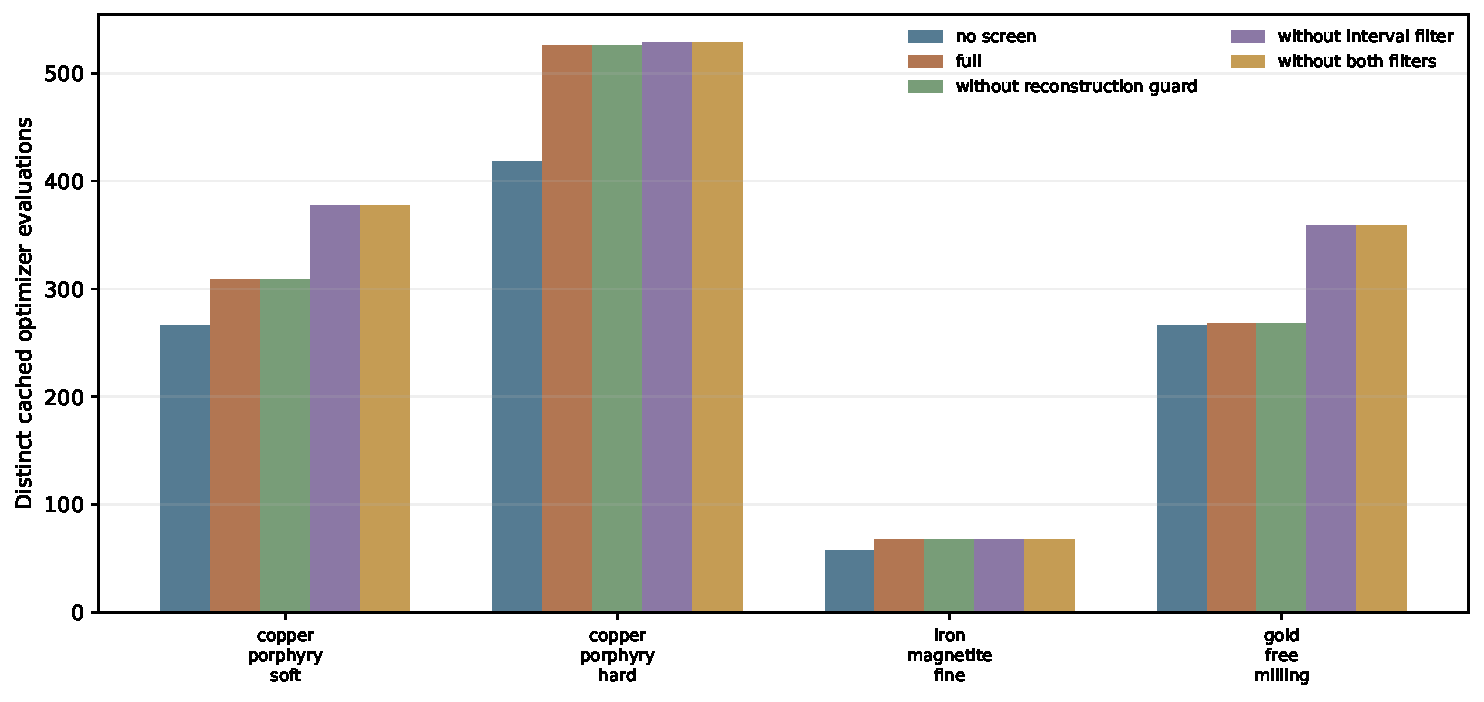
\includegraphics[width=0.92\textwidth]{figures/guard-ablation.pdf}
\caption{Exact evaluation counts for each of five filter policies across four authored cases selected to span distinct circuit configurations.}
\label{fig:guard-ablation}
\end{figure}

\begin{table}[htbp]
\centering
\small
\caption{Paired search outcomes for the 72 authored target-mode variants, using distinct cached exact-engine trial states as the cost measure.}
\label{tab:paired}
\begin{tabular}{lr}
\toprule
Measure & Result \\
\midrule
Paired variants & 72 \\
Screened evaluations & 26367 \\
Unscreened evaluations & 22487 \\
Change & +17.25\% \\
Case-cluster bootstrap 95\% interval for change & [9.28, 25.88]\% \\
Higher / tied / lower cost & 68 / 4 / 0 \\
Same terminal outcome & 65 / 72 \\
Case-cluster bootstrap 95\% interval for agreement & [80.6, 98.6]\% \\
Median recovered-metal difference (t/h) & 0.000000 \\
Maximum recovered-metal difference (t/h) & 0.002653 \\
\bottomrule
\end{tabular}
\end{table}

\begin{table}[htbp]
\centering
\small
\caption{Evaluation counts aggregated by the four authored circuit families; every family retains its number of paired target-mode variants.}
\label{tab:families}
\begin{tabular}{lrrrr}
\toprule
Circuit family & Variants & Unscreened & Screened & Change (\%) \\
\midrule
deslime\_rougher & 18 & 6240 & 6697 & 7.32 \\
gravity\_rougher & 6 & 1616 & 1635 & 1.18 \\
magnetic & 6 & 312 & 373 & 19.55 \\
rougher & 42 & 14319 & 17662 & 23.35 \\
\bottomrule
\end{tabular}
\end{table}

\begin{table}[htbp]
\centering
\small
\caption{Nominal weight-one search ablation on twelve authored cases, isolating candidate distance from the matched unscreened baseline.}
\label{tab:ablation}
\begin{tabular}{lrrrr}
\toprule
Screen policy & Cases & Evaluations & Change vs baseline & Same recovered metal \\
\midrule
No screen & 12 & 3683 & +0.00\% & 12 \\
One mesh step & 12 & 3753 & +1.90\% & 12 \\
One and two steps & 12 & 3974 & +7.90\% & 11 \\
\bottomrule
\end{tabular}
\end{table}

\begin{table}[htbp]
\centering
\small
\caption{Screen candidate counts and exact proposal diagnostics aggregated from the 72 paired artifacts, including the selected-proposal error distribution.}
\label{tab:screen-events}
\begin{tabular}{lr}
\toprule
Event & Count \\
\midrule
Guard rejections & 19 \\
Interval-width rejections & 48268 \\
Exact proposals & 5811 \\
Proposals improving incumbent & 901 \\
Absolute error median (pp) & 0.483 \\
Mean absolute error (pp), case-cluster 95\% interval & 0.712 [0.487, 0.975] \\
Absolute error 95th percentile (pp) & 1.825 \\
Maximum absolute error (pp) & 38.158 \\
\bottomrule
\end{tabular}
\end{table}

\begin{table}[htbp]
\centering
\small
\caption{Filter-removal ablation totals across four selected authored cases, compared with the matched no-screen policy and exact endpoint agreement.}
\label{tab:guard-summary}
\begin{tabular}{lrrr}
\toprule
Policy & Evaluations & Change vs no screen & Same endpoint \\
\midrule
no screen & 1007 & +0.00\% & 4/4 \\
full & 1171 & +16.29\% & 4/4 \\
without reconstruction guard & 1171 & +16.29\% & 4/4 \\
without interval filter & 1332 & +32.27\% & 4/4 \\
without both filters & 1332 & +32.27\% & 4/4 \\
\bottomrule
\end{tabular}
\end{table}

\begin{table}[htbp]
\centering
\small
\caption{Per-case filter policy outcomes preserve evaluation counts, recovered metal, and endpoint agreement for all twenty matched runs.}
\label{tab:guard-cases}
\begin{tabular}{lrrrr}
\toprule
Authored case & Policy & Evaluations & Recovered metal (t/h) & Endpoint \\
\midrule
copper porphyry soft & no screen & 266 & 5.195311 & same \\
copper porphyry soft & full & 309 & 5.195311 & same \\
copper porphyry soft & without reconstruction guard & 309 & 5.195311 & same \\
copper porphyry soft & without interval filter & 377 & 5.195311 & same \\
copper porphyry soft & without both filters & 377 & 5.195311 & same \\
copper porphyry hard & no screen & 418 & 2.548871 & same \\
copper porphyry hard & full & 526 & 2.548871 & same \\
copper porphyry hard & without reconstruction guard & 526 & 2.548871 & same \\
copper porphyry hard & without interval filter & 528 & 2.548871 & same \\
copper porphyry hard & without both filters & 528 & 2.548871 & same \\
iron magnetite fine & no screen & 57 & 232.893406 & same \\
iron magnetite fine & full & 68 & 232.893406 & same \\
iron magnetite fine & without reconstruction guard & 68 & 232.893406 & same \\
iron magnetite fine & without interval filter & 68 & 232.893406 & same \\
iron magnetite fine & without both filters & 68 & 232.893406 & same \\
gold free milling & no screen & 266 & 0.000878 & same \\
gold free milling & full & 268 & 0.000878 & same \\
gold free milling & without reconstruction guard & 268 & 0.000878 & same \\
gold free milling & without interval filter & 359 & 0.000878 & same \\
gold free milling & without both filters & 359 & 0.000878 & same \\
\bottomrule
\end{tabular}
\end{table}
